% !TeX root = ../../main.tex
% Add the above to each chapter to make compiling the PDF easier in some editors.

\section{Generalization over users}\label{ord:ch5:sec_3_generalization_user}

% RE-1468
A challenge for all studies with user interaction are the users themselves, because users of have different levels of knowledge and can therefore be biased.
This is also true for the application of methods, where the performance of the methods should similar different users.
In this study 
% Unteschiede bei verschiedenen Usern sind nicht vermeidbar -> unterschieldiches Level an Erfahrung, unters. Motivation bzw. Verständnis für Genauigkeit und 'wann man fertig ist'.
In this study, participants are biased by different levels of experience, understanding of accuracy, professional background, and motivation.

% Ziel = Methode zu finden mit der alles User gut klarkommen und die über verschiedene user gute Resultate in Zeit und IoU erziehlt.
In order to find wide application, an interactive method must work consistently even with diverse users.
This section examines the generalization capabilities of the benchmark methods across different users and therefore, is the counterpart to the previous section.
% Motivation: generalization over user -> an interactive method really performs well and reliable if it delivers good results for all possible users.


\subsection{Benchmark Participants Evaluation}\label{ord:ch5:sec3:subsec1}

In the following the performance of the methods is evaluated over the \getNumberBenchmarkParticipants \space participants is evaluated.
In contrast to the previous evaluation, here the benchmark runs performed by the colleagues, who are working on this topic, are excluded.
This is done intentionally, in order to not distort the evaluation, since the users are explicitly evaluated here and these experienced users would be strongly biased.

In order to evaluate the generalization capabilities across multiple users, first statistical key figures as the mean and standard deviation $ \sigma $ are evaluated.
The combined mean and $ \sigma $ for the participants are presented in Table \ref{tab:ch5:all_benchmark_users_varaince}.
% For IoU low std-dev, but for time vergleichsweise hoch 
It can be observed, that $ \sigma_{IoU} $ is very similar for the benchmark methods and only ranges from $ \sigma_{IoU} = 0.1187 $ for \gls{dextr} to $ \sigma_{IoU} = 0.1669 $ for watersheds.
In the opposite $ \sigma_{time} $ shows a strong deviation, with $ \sigma_{time} = 15.0977 $ for \gls{dextr} the deviation is more than double than $ \sigma_{time} = 39.0214 $ for polygon.
The mean value is presented to put $ \sigma $ into context.
A graphical illustration if the deviation of $ IoU $ and $ time $ is already presented in the boxplots from Figure \ref{fig:ch5:sec1:iou_box_plot} and \ref{fig:ch5:sec1:time_box_plot}.
Further. these results support the conclusion of Subsection \ref{ord:ch5:sec1:subsec2} and \ref{ord:ch5:sec1:subsec3}, which state that $ \overline{IoU} $ and $ med(IoU) $ do not differ significantly over the methods, while $ \overline{time} $ and $ med(time) $ do differ over the benchmark methods.
% Calculate the variance for time and iou.
\begin{table}[h!]
	\centering
	\begin{tabular}{l|c c c c}
		\toprule 		
		Method 				& $ Polygon $  	& $ Watershed $ 	& $ DEXTR $ 	& $ IOG $	\\
		\midrule
		$ \overline{IoU} $	& 0.8066 		& 0.8166		 	& 0.8543		& 0.8020	\\
		$ \sigma_{IoU} $	& 0.1287 		& 0.1669		 	& 0.1187 		& 0.1559	\\
		$ \overline{time} $	& 34.399 		& 45.076			& 14.542 		& 18.059	\\
		$ \sigma_{time} $	& 39.021 		& 37.796			& 15.098 		& 17.383	\\
		\bottomrule
	\end{tabular}
	\caption[Mean and standard deviation over benchmark methods]{
		Presentation of the mean and standard deviation $ \sigma $ for $ IoU $ and $ time $.
		It can be seen that $ \sigma_{IoU} $ stays almost constant over the benchmark methods.
		In contrast, $ \sigma_{time} $ differs between the methods.
		The mean value was given for IoU and time to better interpret $ \sigma $.
	}\label{tab:ch5:all_benchmark_users_varaince}	
\end{table}

To get even deeper insights about the generalization across different users, in Figure \ref{fig:ch5:sec3:all_benchmark} the boxplots for $ IoU $ and $ time $ are shown for all single participants.
Here, no statistical tests for equality within the methods were performed, because the visualization already anticipates that there are strong deviations in each method.
These variations of individual users are present in all methods and most likely caused by the different experience levels and how well a user got along with the method.
However, it can be stated that \gls{dextr} has the smallest deviation and is the most constant method over all participants.
This observation applies for the $ IoU $ and $ time $ as evaluated parameter.
In terms of $ time $ the \gls{iog} method has also only few deviations, but varies strongly based on the $ IoU $.

In conclusion, the \gls{dextr} method generalizes best over multiple users based on $ IoU $ and $ time $, while the other models do no achieve a constant performance over various users.

% Boxplot of all BenchmarkParticipants (not experienced user aka me)
\begin{figure} [h!]
	\centering
	\begin{subfigure}[t]{1.0\textwidth}
		\centering
		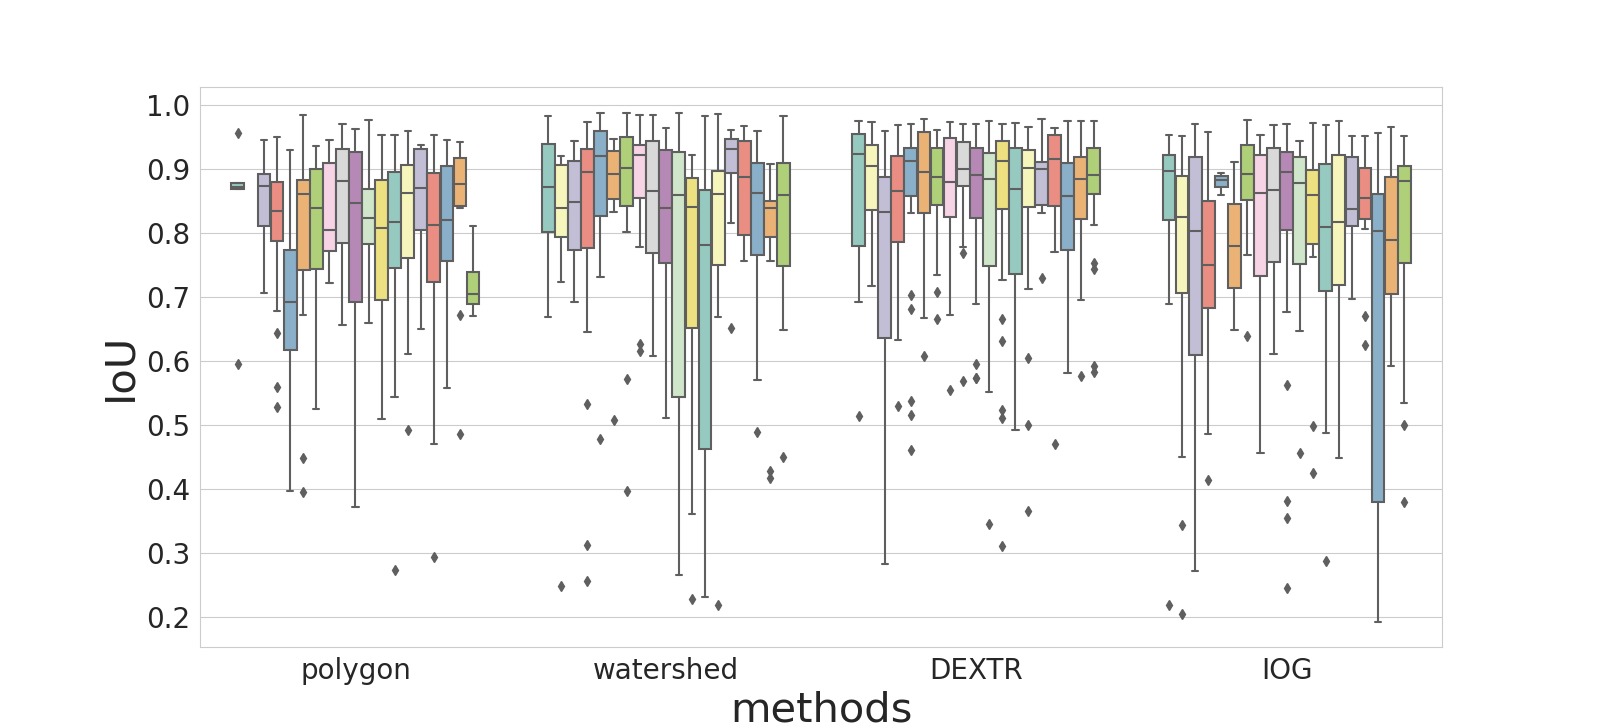
\includegraphics[width=\textwidth]{figures/chap53_all_users_iou.png}
		\caption{
			The \gls{dextr} delivers mostly constant $ IoU $ values with some outliers, while the other methods are mostly characterized by irregularities.
		}\label{fig:ch5:sec3:all_benchmark_iou}
	\end{subfigure}
	\\
	\begin{subfigure}[t]{1.0\textwidth}
		\centering
		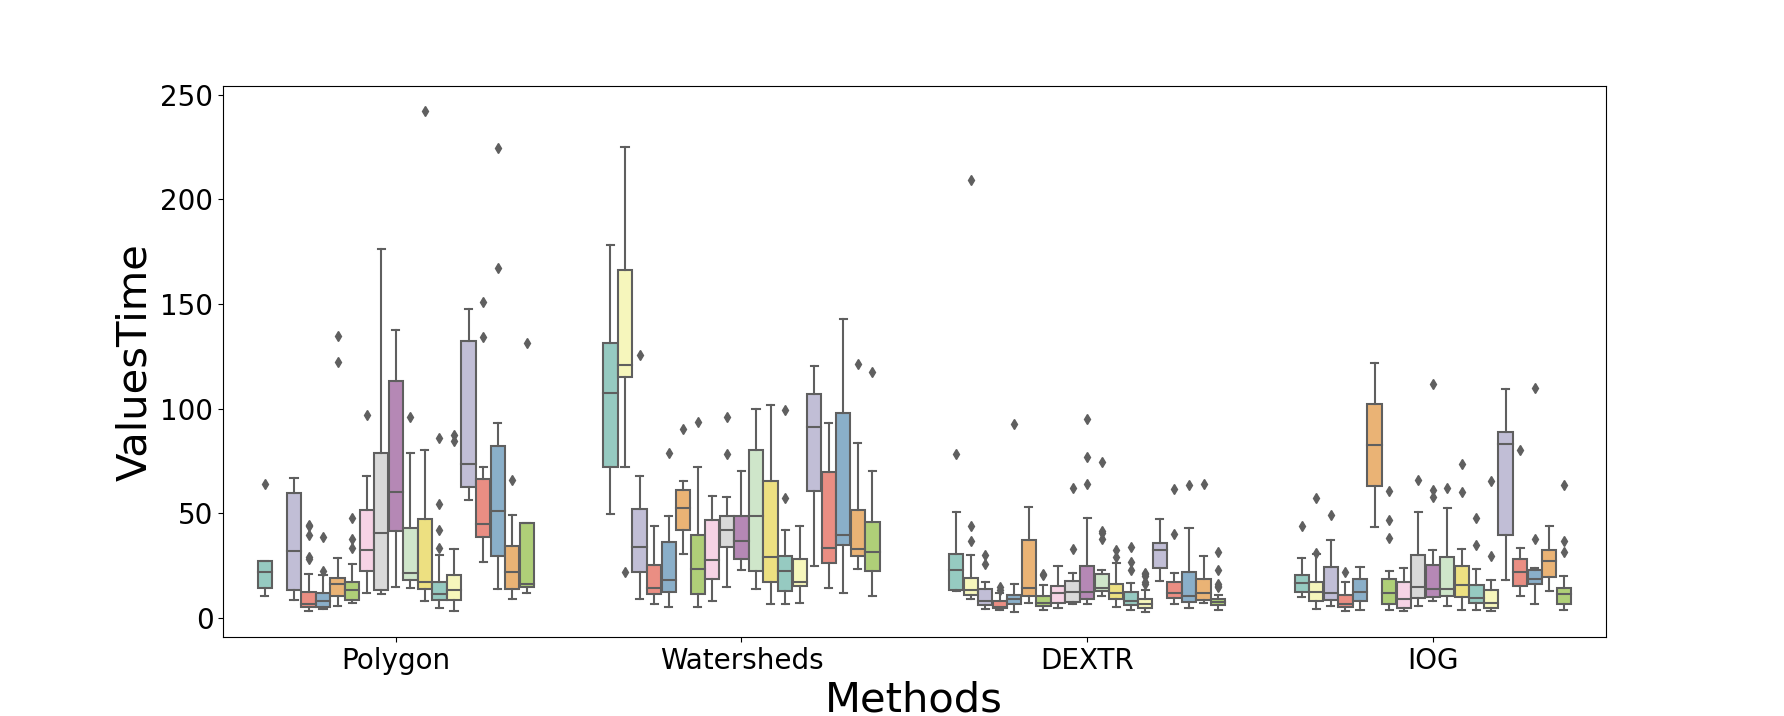
\includegraphics[width=\textwidth]{figures/chap53_all_users_time.png}
		\caption{
			For $ time $ the \gls{dextr} method convinces with constant performance, while the \gls{iog} method has two users who are the exception to the consistency.
			In contrast for the polygon and watershed method consistency over various user is not give.			
		} \label{fig:ch5:sec3:all_benchmark_time}
	\end{subfigure}
	\caption[Boxplots of $ IoU $ and $ time $ over benchmark participants]{		
		The boxplots of $ IoU $ and $ time $ over the \getNumberBenchmarkParticipants \space benchmark participants.
		The single boxplots indicate how the methods performed over the single users. 
		Large differences between the boxplots within a method indicate poor generalization capabilities and vise versa.
	}\label{fig:ch5:sec3:all_benchmark}
\end{figure}

\subsection{Two Experienced User} \label{ord:ch5:sec3:subsec2_cmo_afe}

Normally, the participants have labeled only a part of the benchmark images. 
In the following, eight benchmark runs are evaluated where all benchmark images were labeled by two users who have more experience by working on this topic.
Although only two different users are compared with each other, the significance is given, since all images of the benchmark were labeled.
% Mehrwert dieser Eval - ganzer Benchmark Datensatz wurde durchgemacht
% Big experienced users --> less noise, but still different understandings of being done"


% No significant difference in the IoU between the two user could be detected -> generalize well over various users (few user, large data)
For the $ IoU $ the boxplot in Figure \ref{fig:ch5:sec3:cmo_afe_iou} indicates, that the $ IoU $ is more or less equal over $ \textnormal{\textit{User 1}} $ and $ \textnormal{\textit{User 1}} $ for the four benchmark methods.
The equality of the obtained values from both users are statistically confirmed by the Kruskal-Wallis test, the details of the tests are presented in Table \ref{tab:appendix:afe_cmo_kruskal_wallis_iou}.

An equivalent analysis was performed for $ time $, interestingly here the annotation time between $ \textnormal{\textit{User 1}} $ and $ \textnormal{\textit{User 1}} $ differs strongly for polygon and watershed, while the annotation time is very similar for \gls{dextr} and \gls{iog}.
The statistical relevance is again confirmed by the Kruskal-Walli test, presented in detail in Table \ref{tab:appendix:afe_cmo_kruskal_wallis_time}.

\begin{figure} [h!]
 	\centering
 	\begin{subfigure}[t]{0.49\textwidth}
 		\centering
 		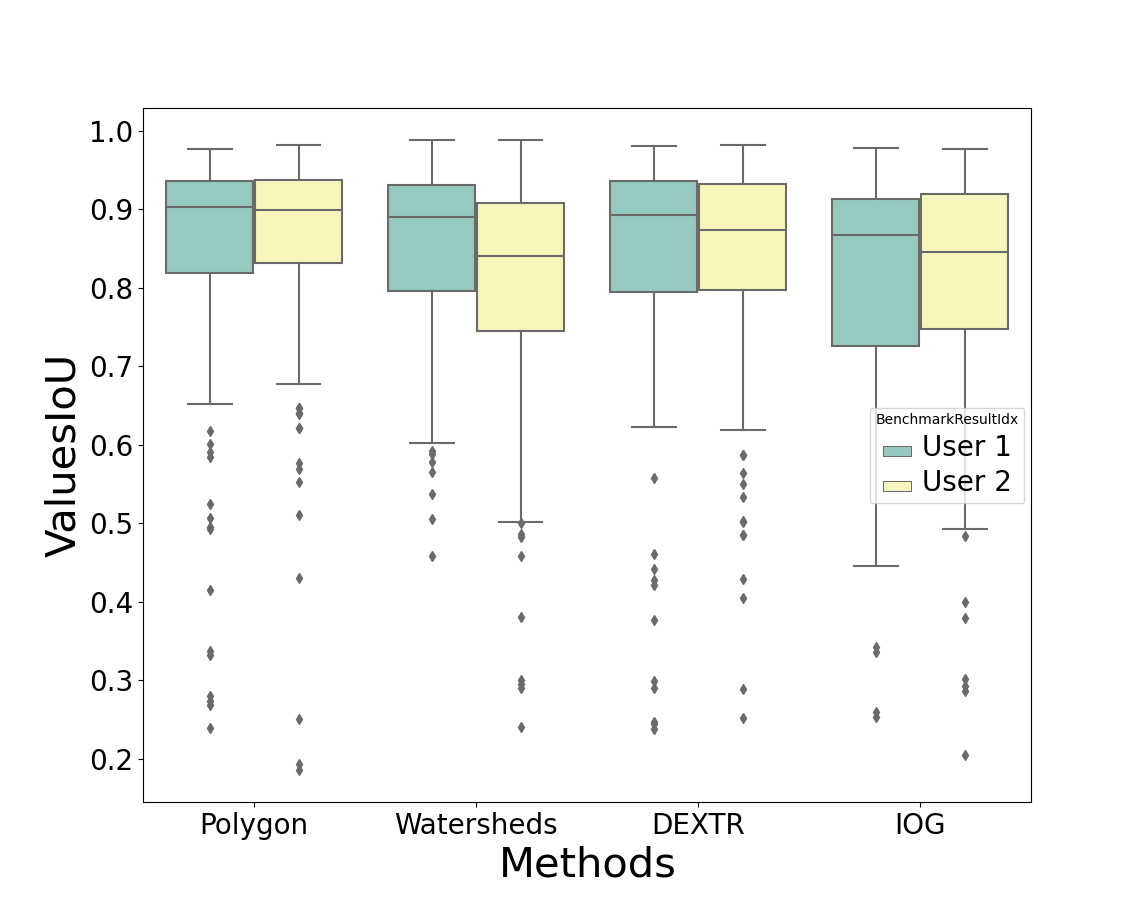
\includegraphics[width=\textwidth]{figures/chap53_afe_cmo_iou.png}
 		\caption{
 			tbd
 		} \label{fig:ch5:sec3:cmo_afe_iou}
 	\end{subfigure}
 	\hfill
 	\begin{subfigure}[t]{0.49\textwidth}
 		\centering
 		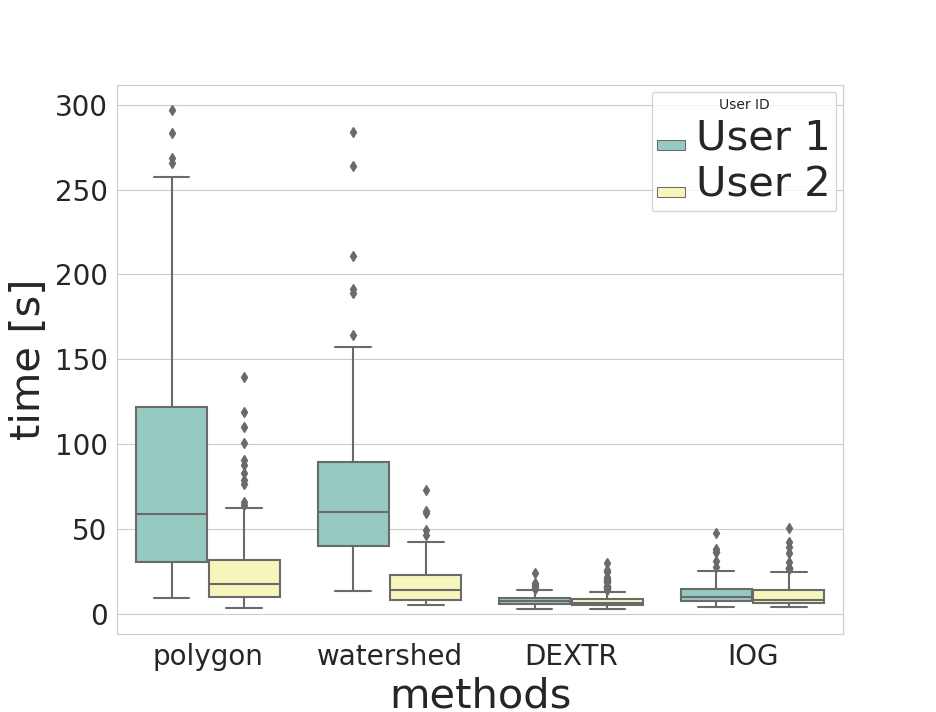
\includegraphics[width=\textwidth]{figures/chap53_afe_cmo_time.png}
 		\caption{
 			tbd
 		}\label{fig:ch5:sec3:cmo_afe_time}
 	\end{subfigure}
 	\caption[IoU Sample Transformation]{		
 		Tbd
 	}\label{fig:ch5:sec3:cmo_afe}
\end{figure}

\subsection{Simulations With Different Click Patterns / Noise}\label{ord:ch5:sec3:subsec3}
% RE-1468

% Simulations are easily scalable, faster and cheaper than the acquisition of manual clicks from real users.
% Second, in a simulation no variance occurs between the set clicks of various users, if the .
% Third, simulations have the possibility to effortless create various click patterns, that \eg vary the set click by a random offset, in order to simulate a various types of user behavior.
%On the other hand, simulations are only capable to replicate the user's behavior to a certain extent.
% Further, the involvement of human users is especially important for methods, which performance depends on user interactions.


In order to gain deeper insights on the functionality of the \gls{dextr} and \gls{iog} method the simulation setup is modified.
% Motivation - Nachahmung von unterschiedlichen Usertypen durch unterschiedliche Genauigkeit bei der Klick-Simulation.
The altered simulation setup uses different levels of accuracy, to simulate more realistic user clicks.
% Simulation of with different permutation / deviation / - simulation of different user

The level of accuracy is defined by a deviation of maximal $ n_{deviation} $ \Unit{px}.
In the range $ \left[-n_{deviation}, \dots, 0, \dots, n_{deviation} \right] $ two values are randomly selected and added to the ideal row and column.
This random factor was added, to simulate the varying accuracy of single user clicks.
The smaller $ n_{deviation} $, the more accurate are the simulated clicks.
In the simulation first the ideal click position is calculated and further the random deviation is added.
This procedure is applied to the extreme points of the \gls{dextr} method and to the fore- and background clicks of the \gls{iog} method.
\begin{table}[h!]
	\centering	
	\resizebox{\textwidth}{!}{
	\begin{tabular}{l l|c c c c c c c}
		\toprule
				&							& \multicolumn{7}{c}{mIoU} \\
				& {$ n_{deviation} $} 		& 0	\Unit{px}	& 5	\Unit{px}	& 10 \Unit{px}	& 15 \Unit{px}	& 20 \Unit{px}	& 25 \Unit{px}	& 30 \Unit{px}	\\
		\midrule
		DEXTR 	& PASCAL (VP \cmark)	& 0.9103	& 0.8323	& 0.7626	& 0.7032 	& 0.6479	& 0.6047	& 0.5626		\\
				& PASCAL (VP \xmark)	& 0.7807	& 0.7523	& 0.7019	& 0.6543 	& 0.6085	& 0.5695	& 0.5317		\\
				& Benchmark			& 0.8414	& 0.7743	& 0.6887	& 0.6240 	& 0.5579	& 0.5027	& 0.4892		\\
		\midrule
		IOG 	& PASCAL (VP \cmark)	& 0.9267	& 0.8846	& 0.8092	& 0.7352 	& 0.6578	& 0.5953 	& 0.5457		\\
				& PASCAL (VP \xmark)	& 0.8081	& 0.7720	& 0.7099	& 0.6476 	& 0.5979	& 0.5337	& 0.4873		\\
				& Benchmark			& 0.8219	& 0.7865	& 0.7173	& 0.6027 	& 0.5268	& 0.4493 	& 0.4058		\\
		\bottomrule
	\end{tabular}}
	\caption[Simulations with different click patterns]{
		Simulations of the \gls{dextr} and \gls{iog} method with user clicks, that are simulated with varying degrees of accuracy.
		The parameter $ n_{deviation} $ states the maximal possible deviation from the optimal point, in order to mimic different types of users.
		As expected, the performance decreases with increasing deviation in the simulated user clicks.
	}\label{tab:ch5:simulation_various_click_patterns}
\end{table}
%TODO benchmark performance of real users for IOG and DEXTR is at 89% and 87% mIoU, while the best simulation is only at 84% and 82% mIoU - das passt nicht so wirklich zusammen.

The performance constantly decreases with higher $ n_{deviation} $, as demonstrated in Table \ref{tab:ch5:simulation_various_click_patterns}. 
Even a comparable small deviation of maximal 5 \Unit{px} leads a notable drop in performance.
This factor needs to be taken into account, if these methods are applied by real users.




